\documentclass[12pt]{article}
\usepackage[margin=25.4mm]{geometry}
\usepackage{graphicx}
\usepackage{hyperref}
\hypersetup{
   colorlinks=true,
   linkcolor=blue,
   filecolor=magenta,
   urlcolor=cyan,
}

\begin{document}
\title{
Adding auxiliary outputs to the YCCC SO2R mini
}
\author{
Kevin Schmidt, W9CF\\
6510 South Roosevelt Street\\
Tempe, Arizona 85283\\
}
\date{}
\maketitle

\section{Introduction}
The YCCC SO2R Mini
\href{https://nn1c.org/so2r/}{https://nn1c.org/so2r/},
as its name implies, is
a small single-operator two-radio interface box which includes the
most important elements needed for interfacing two radios.
Comparing to the more full featured YCCC SO2R+
\href{http://www.k1xm.org/SO2R/}{http://www.k1xm.org/SO2R/}
the Mini, as delivered, does not include LEDs indicating which of the radios
are receiving and which can transmit, manual switches, or auxiliary outputs
that can be interfaced to an antenna switch or band decoder.

The SO2R Mini web site gives information on how to add LEDs and switches
if desired. This document contains my notes on how I added auxiliary
outputs.

\section{Current Mini software and hardware}
The provided Windows connector software supports the OTRSP,
\href{https://www.k1xm.org/OTRSP/index.html}
{\nolinkurl{https://www.k1xm.org/OTRSP/index.html}},
(Open Two-Radio Switching Protocol)
AUX command to provide to two 4 bit auxiliary outputs, i.e. 8 lines total.
It sends a command byte and the auxiliary output byte to the Arduino sketch.
The provided Arduino sketch ignores these, but has a commented define
in the file \verb|keyer_features_and_options.h|
\begin{verbatim}
// #define FEATURE_SO2R_ANTENNA
// SO2R Box antenna selection (not fully implemented)
\end{verbatim}
that turns on detection, and stores the value internally in the code
in \verb|k3ng_keyer.ino|
\begin{verbatim}
    if ((incoming_serial_byte & 0xf0) == 0xa0)
    {
      so2r_antenna_1 = incoming_serial_byte & 0x0f;
      // TBD:  Provide antenna information outputs
      return;
    }
\end{verbatim}
and similarly for the other auxiliary output.

The SO2R Mini designers have done the heavy lifting, so it is straightforward
to add two auxiliary outputs as defined by the OTRSP.

Looking at the Arduino, 8 additional output lines are not available, so
directly connecting Arduino outputs to an auxiliary connector won't work.
However,
the SO2R Mini designers clearly were thinking about making the circuit
expandable and provide various places to mount
headers on the board, and in particular an I$^2$C header for
serial communication is available. I decided to use that to control
an I/O expander to include auxiliary outputs.

\section{My implementation}
I mounted a keyed JST connector to my
SO2R Mini board, but a plane 4 pin header would also work.

There are many I/O expanders available. I first tested with a
Texas instrument PCF8574 since these are readily available.
The problem I found is that while they will sink substantial current,
they can only provide about 100 microamps of source current at 5V.
This was not sufficient for my application, so I decided instead to
use a Microchip
MCP23017. The datasheet is available at
\href{https://ww1.microchip.com/downloads/aemDocuments/documents/APID/ProductDocuments/DataSheets/MCP23017-Data-Sheet-DS20001952.pdf}
{\nolinkurl{https://ww1.microchip.com/downloads/aemDocuments/documents/APID/ProductDocuments/DataSheets/MCP23017-Data-Sheet-DS20001952.pdf}}.


This chip actually has 16 I/O pins, but I only used 8. You could expand
this to all 16 pins easily, the problem is where to mount a 16 or more pin
connector to the SO2R Mini.
You can buy a DIP version of the chip for \$1.69
at Digikey and mount it on a prototype pc board, but I decided to go
with the Adafruit board which has convenient
headers and costs \$5.95. Its available from Digikey
\href{https://www.digikey.com/en/products/detail/adafruit-industries-llc/5346/15913270}
{\nolinkurl{https://www.digikey.com/en/products/detail/adafruit-industries-llc/5346/15913270}}.
You can also buy it directly from Adafruit
\href{https://www.adafruit.com/product/5346}
{\nolinkurl{https://www.adafruit.com/product/5346}}.
The schematic diagram of the board is available at
\href{https://learn.adafruit.com/adafruit-mcp23017-i2c-gpio-expander/downloads}
{\nolinkurl{https://learn.adafruit.com/adafruit-mcp23017-i2c-gpio-expander/downloads}}
which shows how to change the I$^2$C address, etc.

I mounted headers to the Adafruit board for 8 output pins and ground along
with 4 pins to interface with the Mini's I$^2$C port which provides
power and ground along with the I$^2$C clock and data.

\section{Software changes}
As noted above, most of the work has already been done by the SO2R Mini
designers. Adafruit provides a library to use their board, but I think
it is easier to use the Arduino Wire library which is already used in
the K3NG sketch for LCD drivers. Looking at the MCP23017 datasheet,
along with the example code at 
\href{https://www.circuitbasics.com/how-to-use-an-mpc23017-port-expander-on-the-arduino/}
{\nolinkurl{https://www.circuitbasics.com/how-to-use-an-mpc23017-port-expander-on-the-arduino/}},
and noting that the Adafruit board sets the default I$^2$C address
0x20, made everything easy to program. I have provided a patch file with
the changes I made at
\href{file://w9cf.github.io/articles/so2rmini/auxiliary_mcp23017.patch}
{\nolinkurl{auxiliary_mcp23017.patch}}.
I program in linux, so the patch command is always
available there. It can be applied by downloading the sketch from
\href{https://nn1c.org/wp-content/uploads/2020/01/SO2R_Mini_Arduino_Sketch_Configured.zip}
{\nolinkurl{https://nn1c.org/wp-content/uploads/2020/01/SO2R_Mini_Arduino_Sketch_Configured.zip}}
and in linux
\begin{verbatim}
unzip SO2R_Mini_Arduino_Sketch_Configured.zip
patch -p 1 < auxiliary_mcp23017.patch
\end{verbatim}

If you use Windows, and want to patch the code, you can install
git for Windows
\href{https://git-scm.com/download/win}
{\nolinkurl{https://git-scm.com/download/win}}
which includes the
patch executable. You can also make the changes manually as described next.

Changing manually:
\begin{itemize}
\item
In the file \verb|keyer_features_and_options_yccc_so2r_mini.h| uncomment
the line
\begin{verbatim}
// #define FEATURE_SO2R_ANTENNA        // SO2R Box antenna selection (not fully
implemented)
\end{verbatim}
so it reads
\begin{verbatim}
#define FEATURE_SO2R_ANTENNA        // SO2R Box antenna selection
\end{verbatim}
\item
In the file \verb|k3ng_keyer.ino|
\begin{itemize}
\item
At line 2019 change the lines
\begin{verbatim}
  #ifdef FEATURE_SO2R_ANTENNA
    uint8_t so2r_antenna_1 = 0;
    uint8_t so2r_antenna_2 = 0;
  #endif //FEATURE_SO2R_ANTENNA
\end{verbatim}
to
\begin{verbatim}
  #ifdef FEATURE_SO2R_ANTENNA
    #include <Wire.h>
    #define SO2R_ANTENNA_ADDR (0x20) // low low low
    #define SO2R_ANTENNA_GPIOA (0x12)
    #define SO2R_ANTENNA_GPIOB (0x13)
    #define SO2R_ANTENNA_IODIRA (0x00)
    #define SO2R_ANTENNA_IODIRB (0x01)
    uint8_t so2r_antenna_1 = 0;
    uint8_t so2r_antenna_2 = 0;
  #endif //FEATURE_SO2R_ANTENNA
\end{verbatim}
\item
At line 2080 change
\begin{verbatim}
  initialize_sd_card();
\end{verbatim}
to
\begin{verbatim}
  initialize_sd_card();
  initialize_so2r_antenna();
\end{verbatim}
\item
At line 16994 change
\begin{verbatim}
#endif //DEBUG_STARTUP
}


//---------------------------------------------------------------------
\end{verbatim}
to
\begin{verbatim}
#endif //DEBUG_STARTUP
}

void initialize_so2r_antenna() {
#ifdef FEATURE_SO2R_ANTENNA
  Wire.begin();
  #if defined(WIRE_HAS_TIMEOUT)
    Wire.setWireTimeout(10000,true); // 10ms  -- timeout should never occur
  #endif
// Set all 16 pins to outputs, default 0, so they will all be low
// We only use register A 8 pins for SO2R mini
  Wire.beginTransmission(SO2R_ANTENNA_ADDR);
  Wire.write(SO2R_ANTENNA_IODIRA);
  Wire.write(0x00);
  Wire.endTransmission();
  Wire.beginTransmission(SO2R_ANTENNA_ADDR);
  Wire.write(SO2R_ANTENNA_IODIRB);
  Wire.write(0x00);
  Wire.endTransmission();
#endif //FEATURE_SO2R_ANTENNA
}

#ifdef FEATURE_SO2R_ANTENNA
  void update_so2r_antenna() {
    Wire.beginTransmission(SO2R_ANTENNA_ADDR);
    Wire.write(SO2R_ANTENNA_GPIOA);
    Wire.write(((so2r_antenna_2 << 4) | so2r_antenna_1) & 0xff);
    Wire.endTransmission();
  }
#endif //FEATURE_SO2R_ANTENNA


//---------------------------------------------------------------------
\end{verbatim}
\item
At line 21370 and again at line 21377, change
\begin{verbatim}
      // TBD:  Provide antenna information outputs
\end{verbatim}
to
\begin{verbatim}
      update_so2r_antenna();
\end{verbatim}
\end{itemize}
\end{itemize}

At this point, compile and upload the modified sketch. With the
MCP23017 board plugged into the Mini's I$^2$C header ({\em caution,
the order of the 4 wires is not the same on the Mini as on the
Adafruit board -- make sure you have them connected correctly!})
the A0 through A3 outputs should reflect AUX1 and A4 through A8 should
reflect AUX2. If you use N1MM+, these should follow the Antenna assignments.

Once you have the chip working then the hard work of figuring out how
to complete the physical part of the project is left.

\section{My current implementation}

I used double sided tape to secure the Adafruit board to the audio
transformers in the Mini.
I don't think that will 
induce any audio interference, and
I don't hear any so far. It's easy to move if necessary.

After initial testing, I
used a scribe to transfer the hole pattern of the Mini
end plate to a scrap of thin aluminum sheet, and then squeezed in a DB-9
connector carrying the 8 output lines and a common ground. My plan is to
mount the connector on the original Mini end plate after I make sure this
works the way I want it to. Everything I have done so far allows me to
revert to the original Mini.

The MCP23017 mounting and the scrap aluminum end plate with
DB-9  are shown in
Fig. \ref{f1.mcp23017_mount}.
\begin{figure}
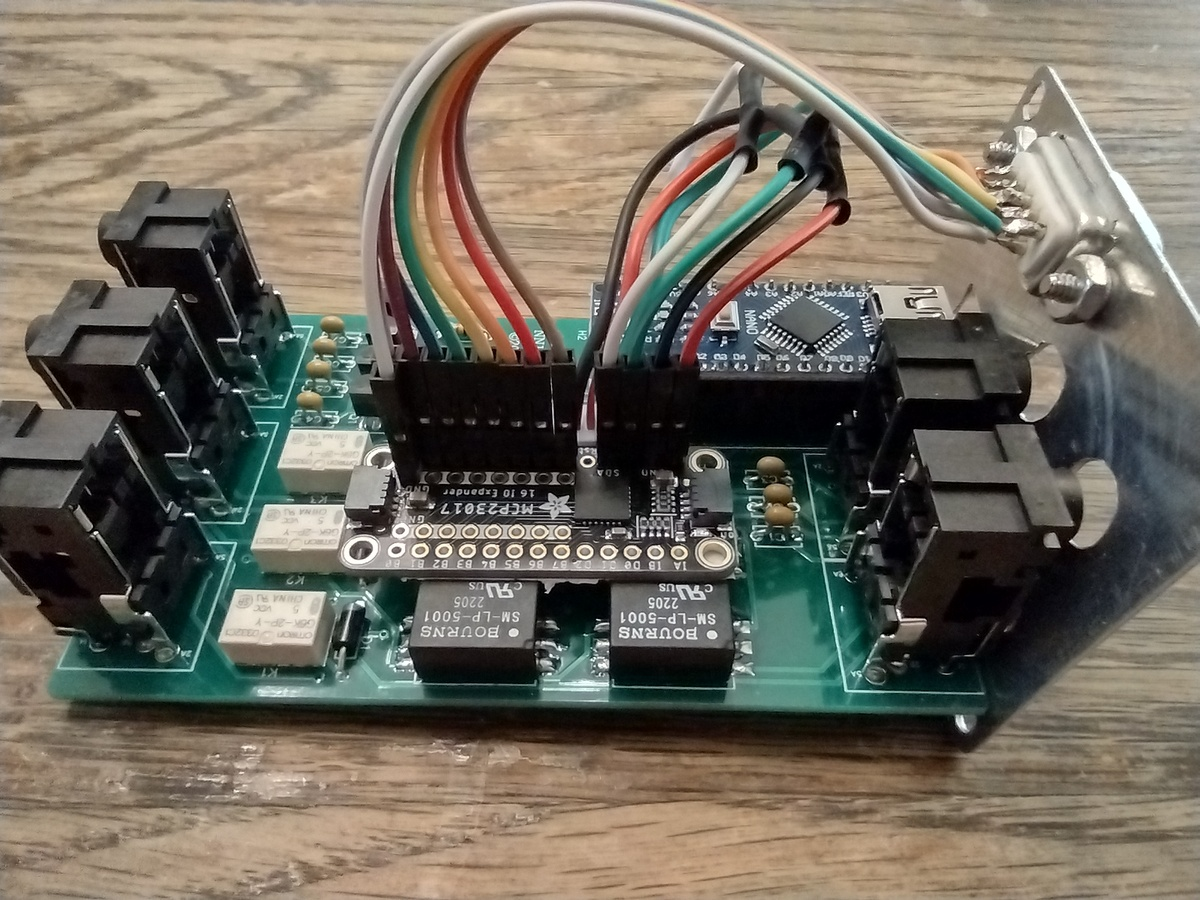
\includegraphics[width=.5\textwidth]{Adafruit_MCP23017_mounted_1.jpg}
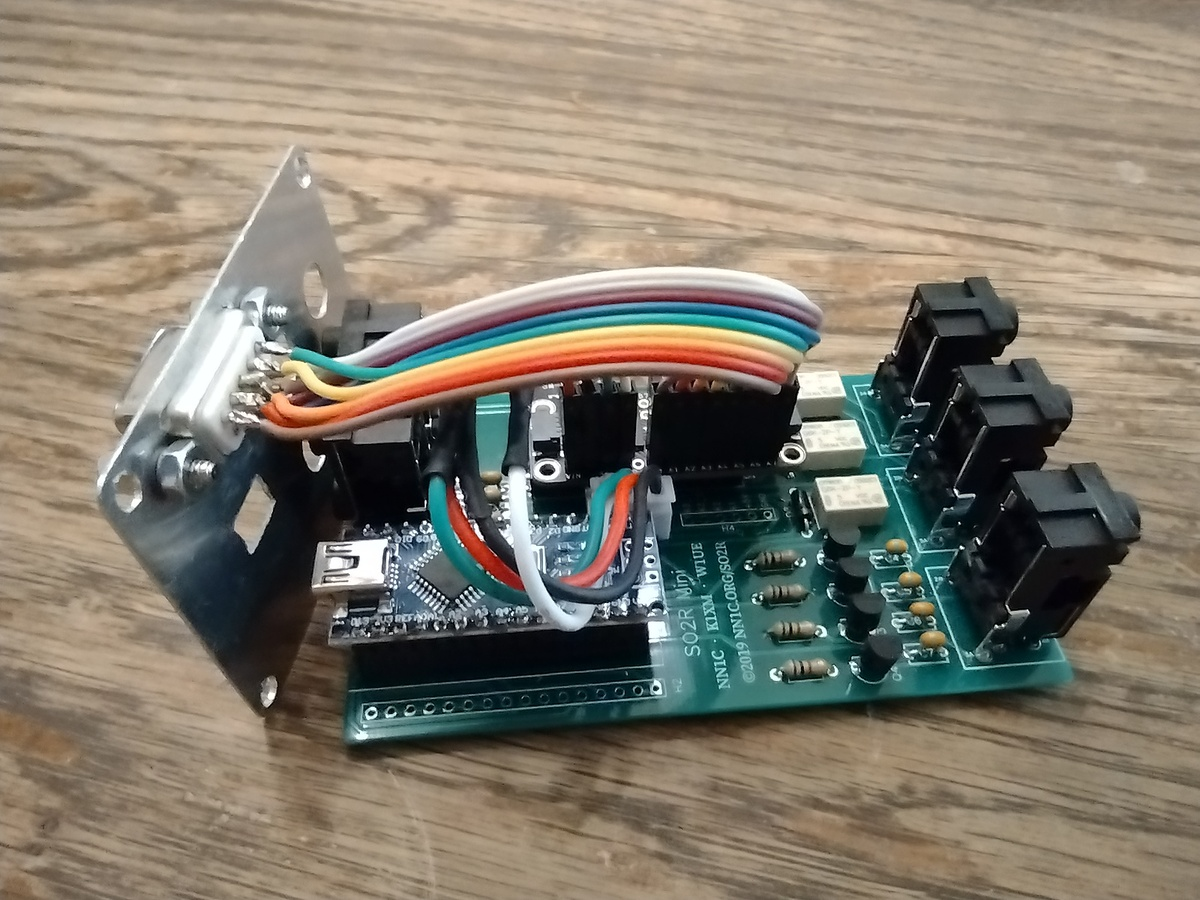
\includegraphics[width=.5\textwidth]{i2c_plug_and_db9_1.jpg}

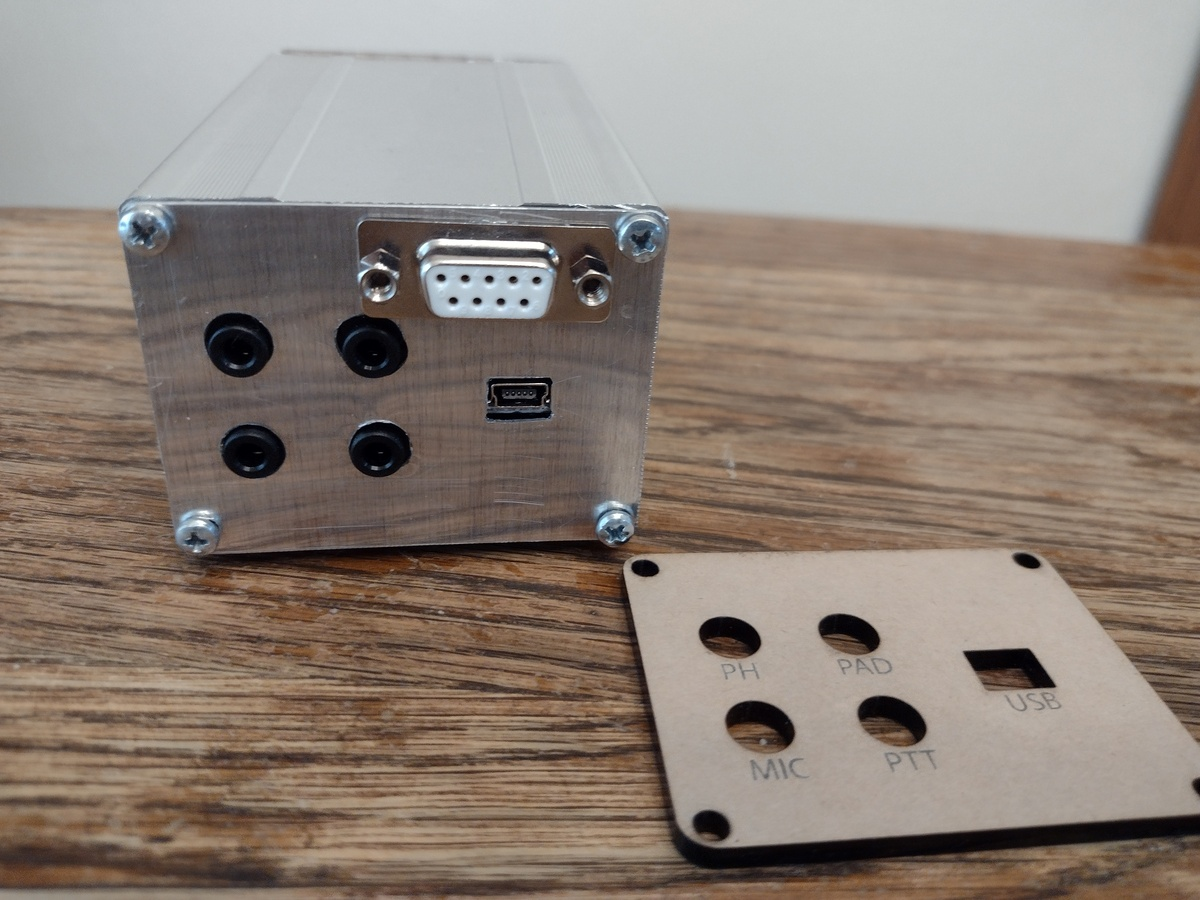
\includegraphics[width=.5\textwidth]{db9_position_1.jpg}
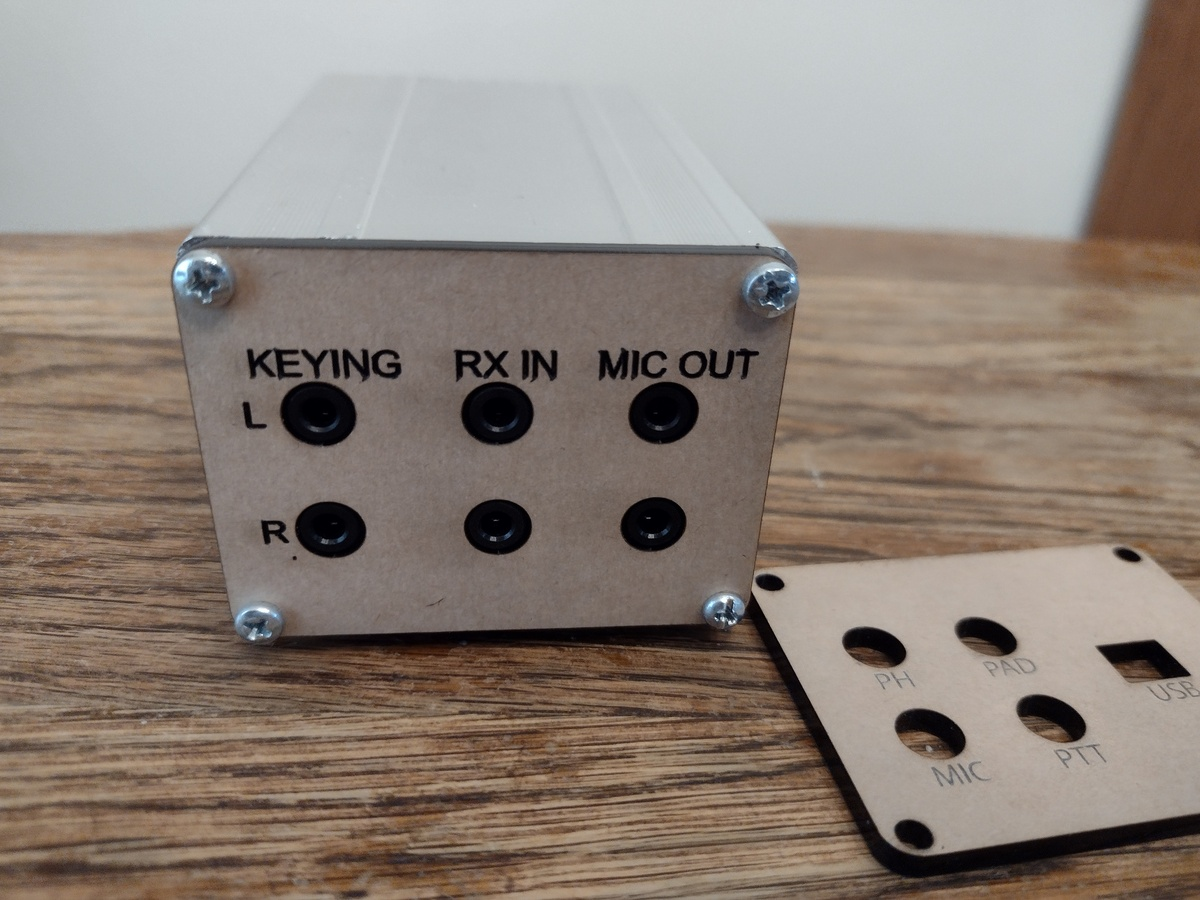
\includegraphics[width=.5\textwidth]{opposite_end_1.jpg}

\caption{Photographs of the SO2R Mini board with the Adafruit MCP23017
board attached with double sided tape and connected to the Mini's
I$^2$C bus and a DB-9 connector.
}
\label{f1.mcp23017_mount}
\end{figure}

As a first test, of my quick and dirty packaging,
I wired a DB-9 male connector to some jumpers and
breadboarded 8-LEDs. These follow the antenna outputs in N1MM+ and
the outputs using TR log in linux as shown in Fig. \ref{f2.leds}.
\begin{figure}
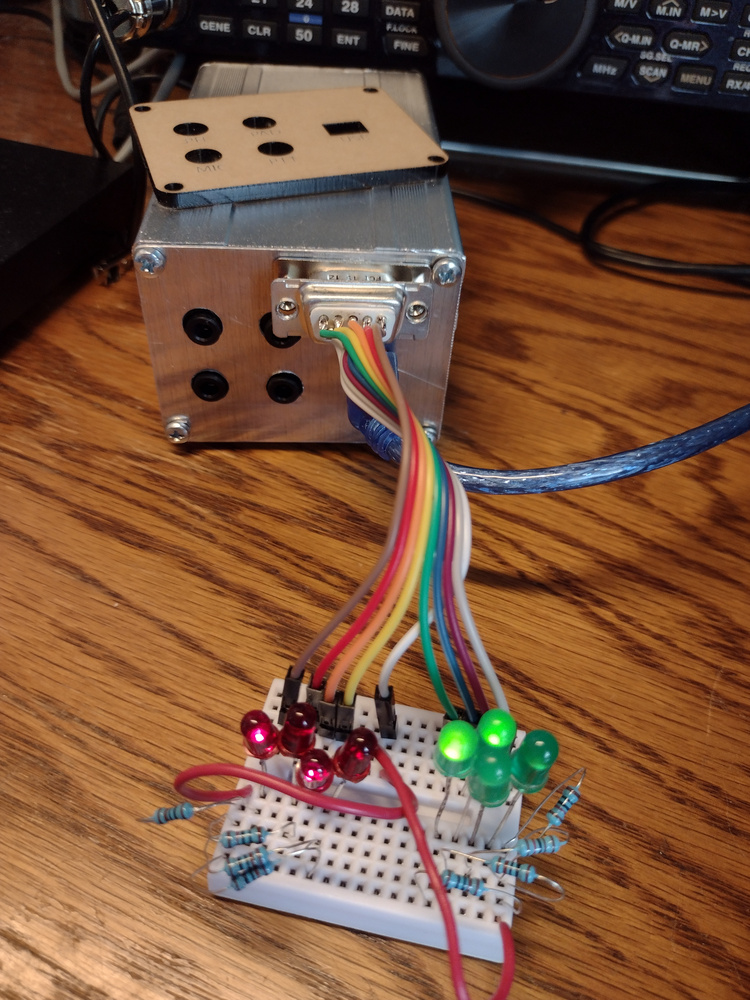
\includegraphics[width=.5\textwidth]{led_test_1.jpg}
\caption{A test showing LEDs following the logging program.}
\label{f2.leds}
\end{figure}

\section{Additional thoughts}
Looking at the YCCC SO2R+ box schematic, the auxiliary output lines there
each have a 220 ohm series current limiting resistor. It would be a good
idea to include those here. I plan to mount them on the DB-9 connector.
In addition, to keep RF out of the Mini, it would also
be a good idea to bypass the DB-9 connections to ground
with 0.01 $\mu$F capacitors.

The DB-9 I used is quite close to the paddle input, so using this mounting,
you may have to choose a slim DB-9 male connector or a right angle
paddle connector to keep from having interference. An alternative connector
with at least 9 connections (8 signal plust ground)
might be a better choice if one can be identified.

\end{document}
